% \pagebreak[4]
% \hspace*{1cm}
% \pagebreak[4]
% \hspace*{1cm}
% \pagebreak[4]

\chapter{Synergy Sansthan}
\ifpdf
    \graphicspath{{Chapter1/Chapter1Figs/PNG/}{Chapter1/Chapter1Figs/PDF/}{Chapter1/Chapter1Figs/}}
\else
    \graphicspath{{Chapter1/Chapter1Figs/EPS/}{Chapter1/Chapter1Figs/}}
\fi

\section{Founders}
\begin{itemize}
	\item \textbf{Mr. Ajay Pandit} \newline
		Mr Ajay Pandit, founder member and Executive Secretary of Synergy Sansthan, belongs to a farmer family. He is 30 year old. His education is MSW, Diploma in Disaster Management \& fellow of National child right fellowship of CRY. Mr. Ajay is also conducting various study like that Process documentation of ``technically support system for SSA'' of MV foundation, Education Micro Plan for Aide et Action etc. He has been working in the voluntary sector for the last 6 years. In the year 2006 he started the activities under the banner of Synergy Sansthan in block Timarni of Harda district in Madhya Pradesh.
	\item \textbf{Mr. Vimal Jat} \newline
		Mr. Vimal Jat, 27 is the President of Synergy Sansthan. His educational background is MSW. He has over 5 years of experience in the social sector. His main areas of focus with Synergy Sansthan are assessing the overall working of different bodies and procuring funds from other NGOs and individuals.
	\item \textbf{Mr. Vishnu Jaiswal} \newline
		Mr. Vishnu Prasad Jaiswal, 28 is the Vice President of Synergy Sansthan. His educational background is MSW,  MBA. He has a lot of experience in the social sector. He belongs to an agriculture based family. He is associated with the child line team of Synergy Sansthan and monitors their activities closely.
\end{itemize}

% Here is an equation\footnote{the notation is explained in the nomenclature section :-)}:
% \begin{eqnarray}
% CIF: \hspace*{5mm}F_0^j(a) &=& \frac{1}{2\pi \iota} \oint_{\gamma} \frac{F_0^j(z)}{z - a} dz
% \end{eqnarray}
% \nomenclature[zcif]{$CIF$}{Cauchy's Integral Formula}                                % first letter Z is for Acronyms 
% \nomenclature[aF]{$F$}{complex function}                                                   % first letter A is for Roman symbols
% \nomenclature[gp]{$\pi$}{ $\simeq 3.14\ldots$}                                             % first letter G is for Greek Symbols
% \nomenclature[gi]{$\iota$}{unit imaginary number $\sqrt{-1}$}                      % first letter G is for Greek Symbols
% \nomenclature[gg]{$\gamma$}{a simply closed curve on a complex plane}  % first letter G is for Greek Symbols
% \nomenclature[xi]{$\oint_\gamma$}{integration around a curve $\gamma$} % first letter X is for Other Symbols
% \nomenclature[rj]{$j$}{superscript index}                                                       % first letter R is for superscripts
% \nomenclature[s0]{$0$}{subscript index}                                                        % first letter S is for subscripts

\section{Vision}
``Promoting intensive participatory process of natural resources development and local institution development. Particular emphasis on unreached, under reached area and women, child, poor and marginalized people.''
\newline
``To create a healthy, educated, free from exploitation, equal harmony and peaceful society''

\section{Objectives}
\begin{itemize}
	\item To promote education, participation awareness, health and nutrition the use of science and technology based on traditional pattern, ecological farming and sustainable livelihood systems.
	\item To promote activities focused on the development of the women, children, Back ward Class, Dalits \& tribal communities.
	\item To work for the communities in such a way that they develop spirit for mutual co-operation, participation, gender equity and justice
\end{itemize}

\section{Funding}
	Synergy Sansthan receives funding from different organizations and people for different projects. Some projects which are conducted under bigger NGOs like the Entrepreneurship Development Program conducted through the NGO Pravah, get funding from Pravah. Some projects like the child line get funding from Child Line, Mumbai. The Asha Training program gets funding from the National Rural Health Mission. Other sources include voluntary donations by individuals and organizations.
% \subsection{sub first paragraph}
% ... and some more ...

% Now I would like to cite the following: \cite{latex} and \cite{texbook}
% and \cite{Rud73}.

% I would also like to include a picture ...

% \begin{figure}[!htbp]
%   \begin{center}
%     \leavevmode
%     \ifpdf
%       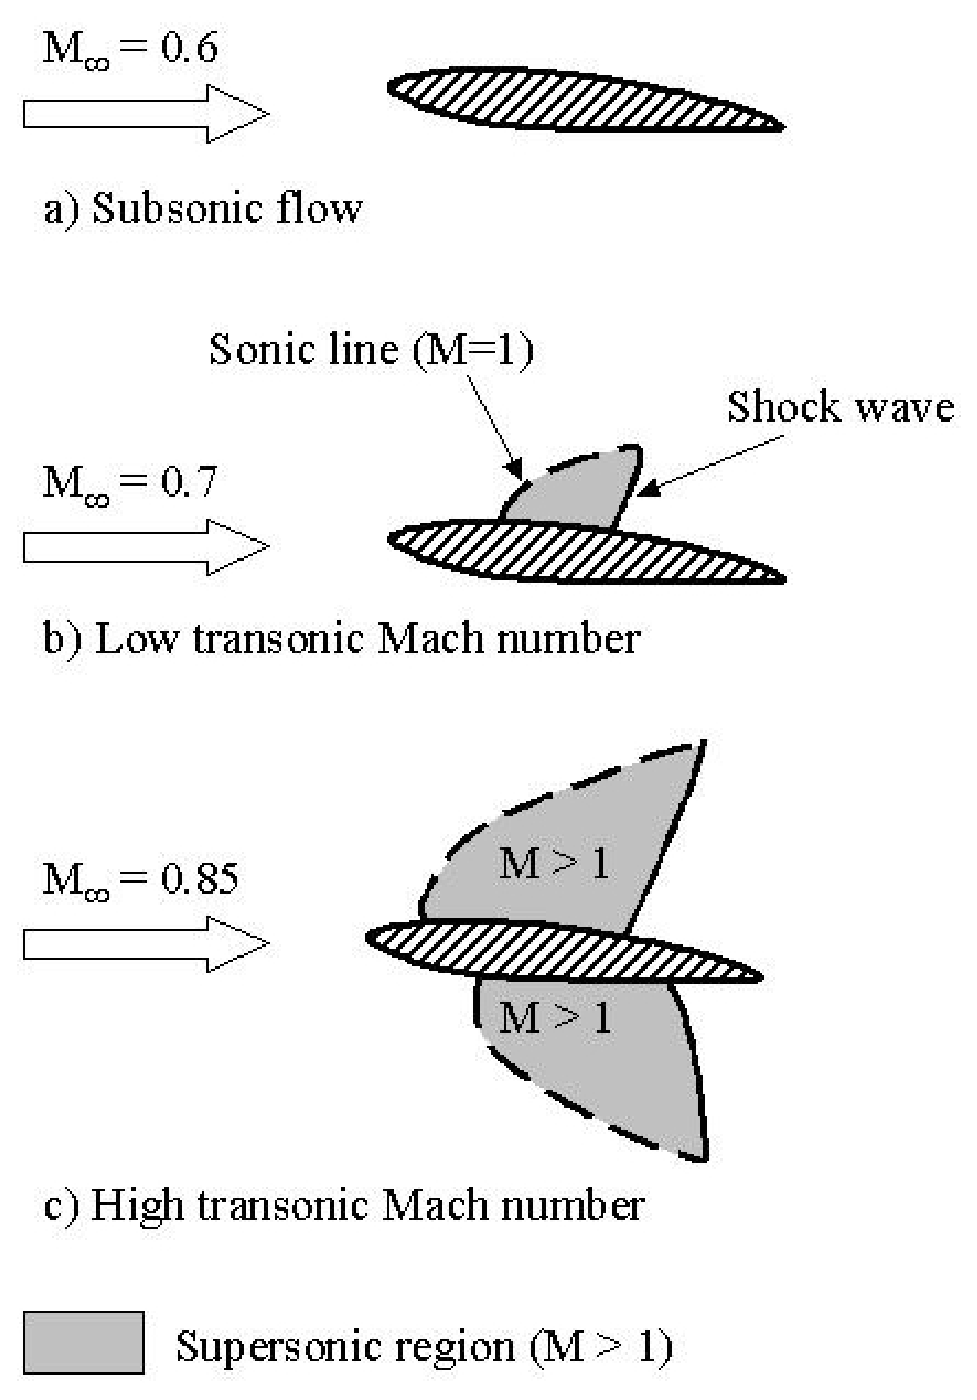
\includegraphics[height=6in]{aflow}
%     \else
%       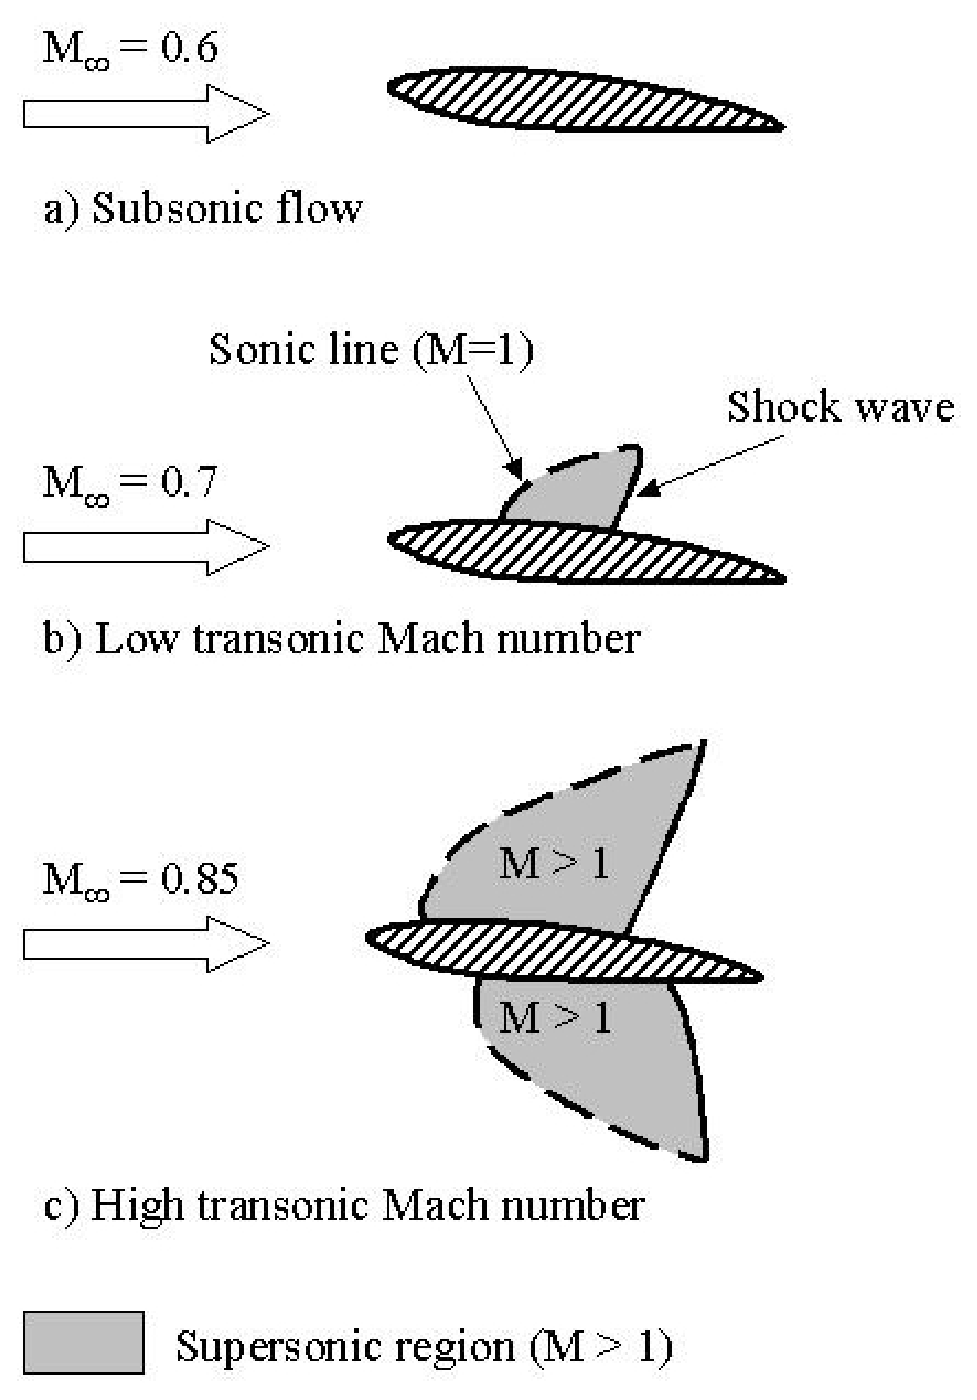
\includegraphics[bb = 92 86 545 742, height=6in]{aflow}
%     \fi
%     \caption{Airfoil Picture}
%     \label{FigAir}
%   \end{center}
% \end{figure}

% above code has been macro-fied in Classes/MacroFile.tex file
%\InsertFig{\IncludeGraphicsH{aflow}{6in}{92 86 545 742}}{Airfoil Picture}{FigAir}

% So as we have now labelled it we can reference it, like so (\ref{FigAir}) and it
% is on Page \pageref{FigAir}. And as we can see, it is a very nice picture and we
% can talk about it all we want and when we are tired we can move on to the next
% chapter ...

% I would also like to add an extra bookmark in acroread like so ...
% \ifpdf
%   \pdfbookmark[2]{bookmark text is here}{And this is what I want bookmarked}
% \fi
% ------------------------------------------------------------------------


%%% Local Variables: 
%%% mode: latex
%%% TeX-master: "../thesis"
%%% End: 
